\documentclass[12pt,a4paper]{article}

\usepackage[T1]{fontenc}
\usepackage[utf8]{inputenc}
\usepackage[brazil]{babel}
\usepackage{graphicx}
\usepackage{geometry}
\usepackage{listings}
\usepackage{listingsutf8}
\usepackage{xcolor}
\usepackage{setspace}
\usepackage{float}
\usepackage{tikz}
\usepackage{tabularx}

\usetikzlibrary{positioning, shapes.geometric}
\onehalfspacing
\geometry{margin=2.5cm}

\lstset{
    language=SQL,
    basicstyle=\ttfamily\small,
    keywordstyle=\color{blue},
    commentstyle=\color{gray},
    stringstyle=\color{red},
    breaklines=true,
    showstringspaces=false
}

\newcommand{\montarinicio}[3]{
    % =========================
    % CAPA
    % =========================
    \begin{titlepage}
        \centering

        {\large Faculdade Anhanguera}\\[0.5cm]
        {\large Tecnólogo em DevOps}\\[3cm]

        {\Large \textbf{#1}}\\[2cm]

        {\large Gabriel Blank Stift Mousquer}\\[1cm]

        {\large Ivoti/RS}\\
        {\large 2026}

    \end{titlepage}

    % =========================
    % FOLHA DE ROSTO
    % =========================
    \begin{titlepage}
        \centering

        {\large Faculdade Anhanguera}\\[0.5cm]
        {\large Tecnólogo em DevOps}\\[2cm]

        {\Large \textbf{#1}}\\[1.5cm]

        \begin{flushright}
            Trabalho apresentado à disciplina de \\
            \textbf{#2} \\
            Professor: #3 \\
        \end{flushright}

        \vfill

        {\large Gabriel Blank Stift Mousquer}\\
        Matrícula: 2024201126\\

        \vfill

        {\large Ivoti/RS}\\
        {\large 2026}

    \end{titlepage}

    % =========================
    % SEÇÃO: TOC
    % =========================
    \tableofcontents
    \newpage
}


\begin{document}

\montarinicio
    {CRIANDO UMA MODELAGEM DE DADOS}
    {Programação e Desenvolvimento de Banco de Dados}
    {Thaysla Fernanda Da Cruz Cardoso}

% =========================
% SEÇÃO: INTRODUÇÃO
% =========================
\section{Introdução}

O presente trabalho tem como objetivo demonstrar a utilização de comandos SQL no contexto de criação e manipulação de uma base de dados relacional, conforme proposto na atividade prática. Em particular, busca-se aplicar comandos de definição de dados (\textit{DDL}) para a construção da estrutura de um banco de dados a partir de um diagrama entidade-relacionamento, bem como comandos de manipulação (\textit{DML}) e consulta (\textit{DQL}) para inserção e recuperação de dados.

Foi implementada a estrutura da base de dados a partir do diagrama entidade-relacionamento fornecido. A modelagem foi traduzida para comandos SQL, respeitando as entidades, atributos e relacionamentos definidos no DER.

Em seguida, foram realizadas operações de inserção de dados nas tabelas criadas, com o objetivo de popular a base para testes e validação das estruturas implementadas. Cada tabela recebeu ao menos três registros, conforme solicitado na atividade.

Também foi definida uma visão (\textit{VIEW}) responsável por retornar todas as contas com situação igual a 1, representando as contas ainda não pagas, permitindo a consulta filtrada dos dados armazenados.

As atividades foram realizadas em um ambiente baseado no sistema operacional \textit{Ubuntu 24.04.4 LTS}, utilizando o SGBD \textit{MySQL}, versão 8.0.45, acessado por meio da interface de linha de comando (CLI). O acesso ao banco foi realizado com o usuário \texttt{aula1}, por meio do comando \texttt{mysql -u aula1 -p}.

% =========================
% SEÇÃO: DESENVOLVIMENTO
% =========================
\section{Desenvolvimento}

\subsection{Criação das tabelas}

Nesta etapa foi realizada a implementação da estrutura do banco de dados a partir do modelo entidade-relacionamento fornecido. Foram criadas as tabelas necessárias para representar as entidades do sistema, incluindo suas chaves primárias e estrangeiras, de forma a garantir a integridade referencial entre os dados.

\begin{figure}[H]
    \centering
    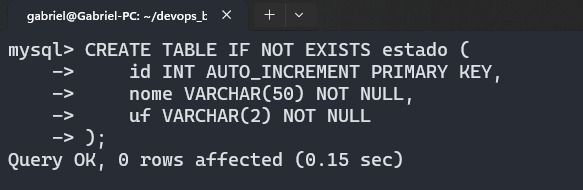
\includegraphics[width=0.8\textwidth]{./static/0-tabela-estado.png}
    \caption{Criação da tabela estado}
    \label{fig:tabela-estado}
\end{figure}

\begin{figure}[H]
    \centering
    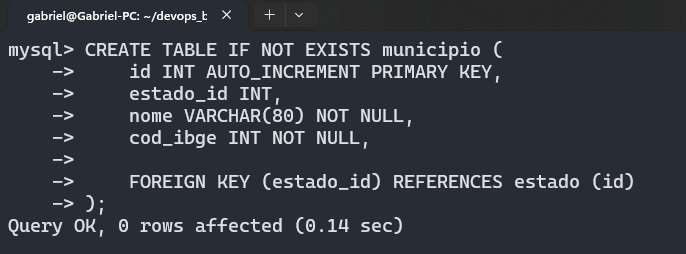
\includegraphics[width=0.8\textwidth]{./static/1-tabela-municipio.png}
    \caption{Criação da tabela municipio}
    \label{fig:tabela-municipio}
\end{figure}

\begin{figure}[H]
    \centering
    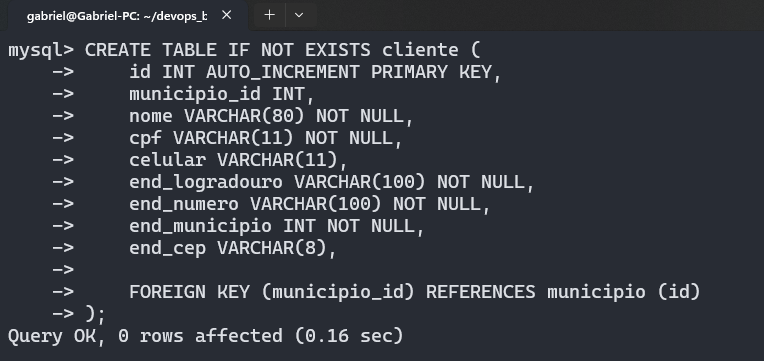
\includegraphics[width=0.8\textwidth]{./static/2-tabela-cliente.png}
    \caption{Criação da tabela cliente}
    \label{fig:tabela-cliente}
\end{figure}

\begin{figure}[H]
    \centering
    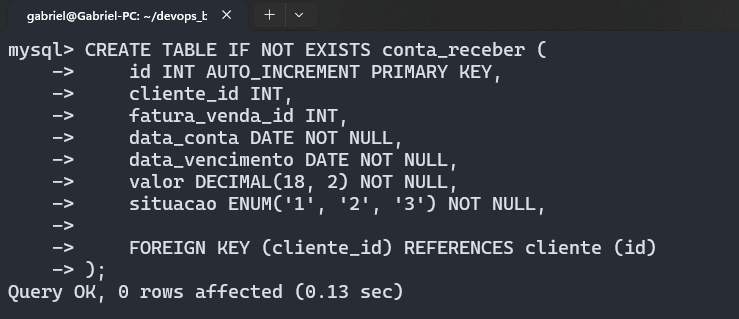
\includegraphics[width=0.8\textwidth]{./static/3-tabela-conta_receber.png}
    \caption{Criação da tabela conta\_receber}
    \label{fig:tabela-conta_receber}
\end{figure}

\subsection{Massa de dados}

Após a criação das tabelas, foi realizada a inserção de registros em cada uma delas, com o objetivo de popular a base de dados e permitir a validação do modelo implementado. Cada tabela recebeu pelo menos três registros, respeitando os relacionamentos definidos na estrutura do banco.

\begin{figure}[H]
    \centering
    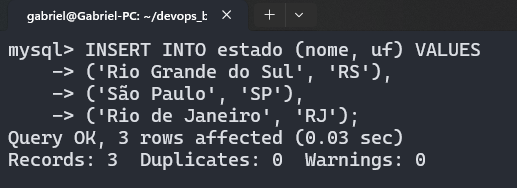
\includegraphics[width=0.8\textwidth]{./static/4-inserir-estado.png}
    \caption{Inserção de dados na tabela estado}
    \label{fig:inserir-estado}
\end{figure}

\begin{figure}[H]
    \centering
    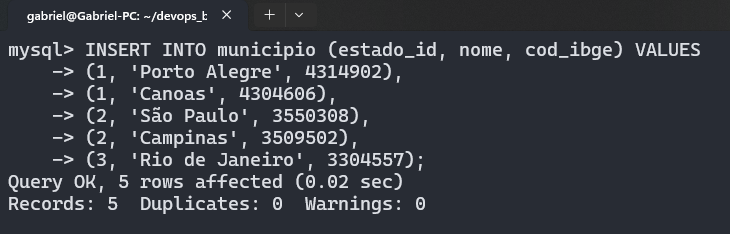
\includegraphics[width=0.8\textwidth]{./static/5-inserir-municipio.png}
    \caption{Inserção de dados na tabela municipio}
    \label{fig:inserir-municipio}
\end{figure}

\begin{figure}[H]
    \centering
    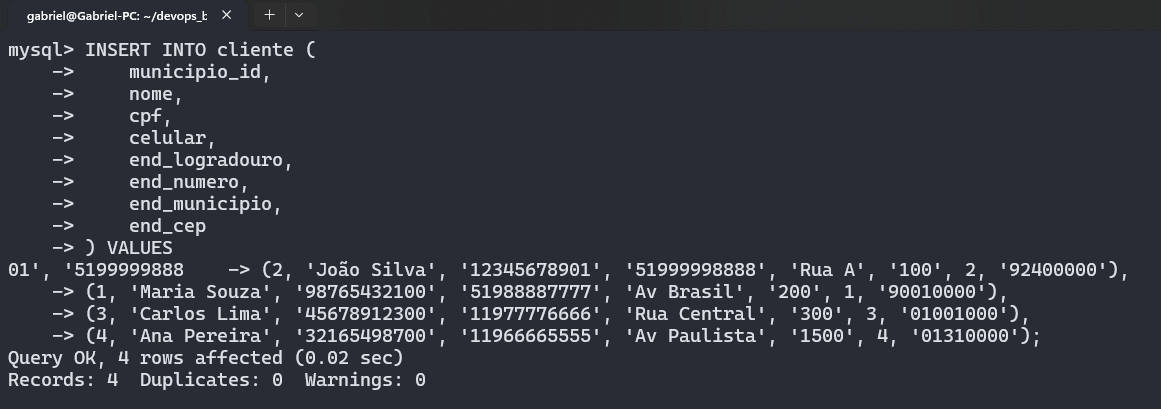
\includegraphics[width=0.8\textwidth]{./static/6-inserir-cliente.png}
    \caption{Inserção de dados na tabela cliente}
    \label{fig:inserir-cliente}
\end{figure}

\begin{figure}[H]
    \centering
    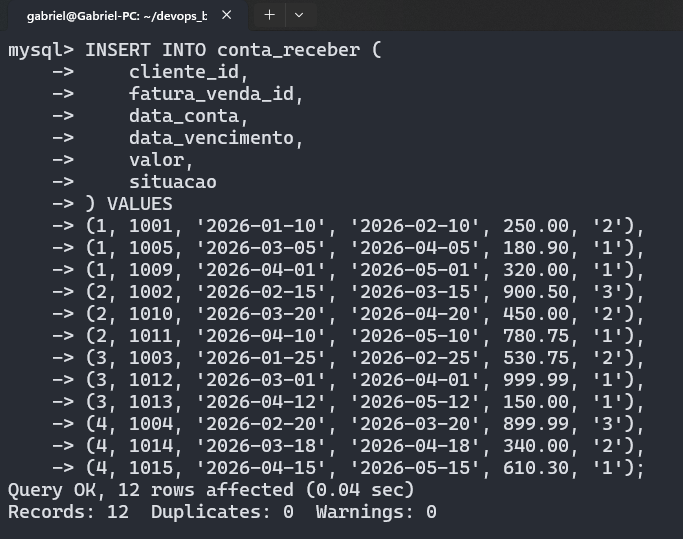
\includegraphics[width=0.8\textwidth]{./static/7-inserir-conta_receber.png}
    \caption{Inserção de dados na tabela conta\_receber}
    \label{fig:inserir-conta_receber}
\end{figure}

\subsection{Criação da view}

Nesta etapa foi definida uma visão (\textit{VIEW}) com o objetivo de facilitar a consulta de dados específicos do sistema. A view foi construída para retornar todas as contas com situação igual a 1, representando as contas pendentes de pagamento, permitindo uma consulta simplificada e centralizada dessas informações.

\begin{figure}[H]
    \centering
    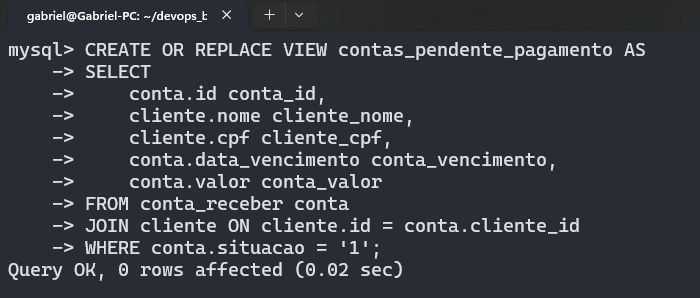
\includegraphics[width=0.8\textwidth]{./static/8-criar-view.png}
    \caption{Criação da view contas\_pendente\_pagamento}
    \label{fig:criar-view}
\end{figure}

\begin{figure}[H]
    \centering
    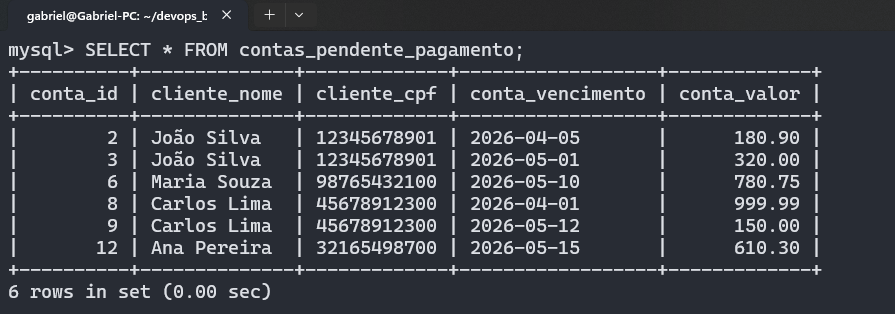
\includegraphics[width=0.8\textwidth]{./static/9-testar-view.png}
    \caption{Exemplo de uso da view contas\_pendente\_pagamento}
    \label{fig:testar-view}
\end{figure}

% =========================
% SEÇÃO: CONCLUSÃO
% =========================
\section{Conclusão}

A realização da atividade permitiu aplicar, na prática, comandos SQL voltados à criação de estruturas de banco de dados a partir de um modelo entidade-relacionamento, bem como à inserção e consulta de dados em um sistema relacional.

Durante o desenvolvimento, observou-se a importância da correta tradução do modelo conceitual (DER) para o modelo físico, garantindo que as entidades, atributos e relacionamentos fossem representados de forma coerente na implementação em SQL. Esse processo é fundamental para assegurar a integridade e a organização dos dados armazenados.

A etapa de inserção de registros possibilitou a validação das estruturas criadas, enquanto a utilização de uma visão (\textit{VIEW}) demonstrou a utilidade de consultas estruturadas para filtragem e organização de informações, facilitando a recuperação de dados específicos do banco.

Dessa forma, a atividade contribuiu para o entendimento prático do processo de modelagem, criação e consulta de bancos de dados relacionais, reforçando a importância do uso adequado de comandos SQL para a construção de sistemas consistentes e funcionais.

% =========================
% SEÇÃO: APÊNDICE
% =========================
\section{Apêndice}

\subsection{Script SQL completo}

\lstinputlisting[
    caption={Script SQL completo},
    label={lst:sql},
    inputencoding=utf8/latin1,
    basicstyle=\ttfamily\scriptsize
]{./static/script.sql}

\end{document}
